\documentclass[12pt]{article}
 \usepackage[margin=1in]{geometry} 
\usepackage{amsmath,amsthm,amssymb,amsfonts}
\usepackage{graphicx}
\usepackage{enumerate}
 
\newcommand{\N}{\mathbb{N}}
\newcommand{\Z}{\mathbb{Z}}
 
\newenvironment{problem}[2][Problem]{\begin{trivlist}
\item[\hskip \labelsep {\bfseries #1}\hskip \labelsep {\bfseries #2.}]}{\end{trivlist}}
%If you want to title your bold things something different just make another thing exactly like this but replace "problem" with the name of the thing you want, like theorem or lemma or whatever

\newenvironment{concept}[1]{\begin{trivlist}
		\item[\hskip \labelsep {\bfseries #1}]}{\end{trivlist}}
 
\begin{document}

 
\title{Machine Learning 101}
\author{Daniel Nguyen}
\maketitle
 
\section{General Data Science}
\begin{concept}{Supervised Learning}
	\
	\begin{itemize}
		\item {
			Process of trying to infer from labeled data the underlying function that produced the labels associated with the data
		}
	\end{itemize}
\end{concept}

\begin{concept}{Unsupervised Learning}
	\
	\begin{itemize}
		\item {
			Find patterns/relationships/structure in data, but are not optimized to solve a particular predictive task
		}
	\end{itemize}
\end{concept}
\begin{concept}{Regression}
	\
	\begin{itemize}
		\item {
			Learn relationships between inputs and outputs
		}
		\item {
			Linear regression uses predictor of the form $X\theta = y$ where $X$ is the matrix of inputs, $y$ is the outputs vector, and $\theta$ is the weights vector.
		}
	\end{itemize}
\end{concept}

\begin{concept}{Mean-squared Error}
	\
	$$E = \frac{1}{N} \sum_{i=1}^{N} (y_i - \boldsymbol{X_i} \cdot \boldsymbol{\theta})^2$$
	\begin{itemize}
		\item {
			What we try to minimize in our regression model
		}
	\end{itemize}

	\textbf{Coefficient of determination ($R^2$ statistic):}
	$$FVU(f) = \frac{MSE(f)}{Var(y)}$$
	
	(FVU = fraction of variance unexplained)
	\begin{itemize}
		\item {
			FVU(f) = 1 - Trivial predictor
		}
		\item {
			FVU(f) = 0 - Perfect predictor
		}
	\end{itemize}
\end{concept}

\begin{concept}{Occam's razor}
	\	
	\begin{itemize}
		\item {
			Among competing hypotheses, the one with the fewest assumptions should be selected
		}
		\item {
			Hypothesis here is our weights $\boldsymbol{\theta}$.
		}
		\item {
			We want $\boldsymbol{\theta}$ with few non-zero parameters, meaning only a few features are relevant, and $\boldsymbol{\theta}$ that is
			almost uniform, meaning only a few features are significantly more relevant than others.
		}
	\end{itemize}
\end{concept}

\begin{concept}{Regularization}
	\
	\begin{itemize}
		\item {
			Process of penalizing the model complexity
		}
	\end{itemize}
	
	\textbf{L2 Regularization}
	$$R(\boldsymbol{\theta}) = \lambda ||\boldsymbol{\theta}||^2_2$$
	
	\begin{itemize}
		\item {
			Regularized model means that we add the regularization term to our model
		}
		\item {
			For example, if we are trying to minimize Sum-squared Error, then the model will become
			$$E = \frac{1}{N} \sum_{i=1}^{N} (y_i - \boldsymbol{X_i} \cdot \theta)^2 + \lambda ||\boldsymbol{\theta}||^2_2$$
		}
	\end{itemize}

	Note: $||\boldsymbol{\theta}||_2 = \sqrt{\sum_{i}^{} \theta_i ^2}$
\end{concept}

\begin{concept}{Data Sets}
	\
	\begin{itemize}
		\item {
			Training Set: used to optimize the model's parameters
		}
		\item {
			Validation Set: used to tune any model parameters that are not directly optimized by the training set
		}
		\item {
			Training Set: used to report how well we expect the model to perform on unseen data
		}
	\end{itemize}
\end{concept}

\begin{concept}{Naive Bayes}
	\
	\begin{itemize}
		\item {
			Assumes that features are conditionally independent given the label, meaning we're assuming
			$$P(feature_i, feature_j | label) = P(feature_i | label) \cdot P(feature_j | label)$$
			where $i \neq j$
		}
		\item {
			Our probability model becomes
			$$P(label | features) = \frac{P(label) \cdot \prod_{i}^{} P(feature_i | label)}{P(features)}$$
		}
		\item {
			Can double count features that are highly correlated (i.e. features that represent the same information) because it makes
			the assumption that each $P(data | label)$ is independent, when it is not.
		}
	\end{itemize}
\end{concept}

\begin{concept}{Logistic Regression}
	\
	\begin{itemize}
		\item {
			Optimize the likelihood of the data by modeling $P(label | data)$. We use a sigmoid function to convert $ \boldsymbol{\theta} \cdot \boldsymbol{x}$ to a probability.
			$$\sigma(t) = \frac{1}{1 + e^{-t}} = P(label | data) = y$$
			where $t = \boldsymbol{\theta} \cdot \boldsymbol{x}$
		}
		\item {
			The Cross-Entropy cost function (what we are trying to minimize) is given by
			$$E(\boldsymbol{\theta}) = - \sum_{n=1}^{N} \left\{ t^n \ln(y^n) + (1-t^n) \ln(1-y^n) \right\}$$
			Note: the $n$ superscript notation refers to the values associated with the input $n$, and not the $n^{th}$ power
		}
		\item {
			The gradient of the cost function with respect to weight $j$ is given by
			$$\frac{\partial E(\boldsymbol{\theta})}{\partial \theta_j} = - \sum_{n=1}^{N} (t^n - y^n) x_j^n$$
		}
		\item {
			Visualized as drawing a line that separates two sets of points.
		}
		\item {
			Tend to overfit with small amount of data
		}
	\end{itemize}
\end{concept}

\begin{concept}{Softmax Regression}
	\
	\begin{itemize}
		\item {
			A probabilistic model, similar to logistic regression; but is able to classify more than two outputs.
		}
		\item {
			$$\sigma(t_i) = \frac{e^{t_i}}{\sum_{k=1}^{c} e^{t_k}} = P(label_i | data) = y_i$$
			where $t_i = \boldsymbol{\theta_i} \cdot \boldsymbol{x}$
		}
		\item {
			The Cross-Entropy cost function (what we are trying to minimize) is given by
			$$E(\boldsymbol{\theta}) = - \sum_{n=1}^{N} \sum_{k=1}^{c} t_k^n \ln(y_k^n)$$
			Note: the $n$ superscript notation refers to the values associated with the input $n$, and not the $n^{th}$ power
		}
		\item {
			The gradient of the cost function with respect to weight $jk$ is given by
			$$\frac{\partial E(\boldsymbol{\theta})}{\partial \theta_{jk}} = - \sum_{n=1}^{N} (t_k^n - y_k^n) x_j^n$$
		}
	\end{itemize}
\end{concept}

\begin{concept}{Support Vector Machine}
	\
	\begin{itemize}
		\item {
			Try to minimize misclassification error using the classifier of the form
			\[
				y_i =
				\begin{cases}
					1 & \boldsymbol{X_i} \cdot \boldsymbol{\theta} - b > 0 \\
					-1 & otherwise
				\end{cases}
			\]
		}
		\item {
			Since we are minimizing the number of misclassifications, we are doing
			$$\arg min_{\boldsymbol{\theta}} \sum_{i}^{} \delta (y_i (\boldsymbol{X_i} \cdot \boldsymbol{\theta} - b) \leq 0)$$
			where the term $\boldsymbol{X_i} \cdot \boldsymbol{\theta} - b$ refers to the model's prediction, $y_i$ is the actual
			label, and $\delta$ is the indicator function that has the value $1$ if the argument is true and $0$ if the argument is false.
			
			We can see that all we're doing here is counting how many were misclassified. If our prediction and label match, we will get
			positive values since we are multiplying them; otherwise, we get negative values.
		}
	\end{itemize}
\end{concept}

\begin{concept}{Classifier Evaluation}
	\
	\begin{itemize}
		\item {
			True Positive (TP): Labeled as T, predicted as T\\
			True Negative (TN): Labeled as F, predicted as F\\
			False Positive (FP): Labeled as F, predicted as T\\
			False Negative (FN): Labeled as T, predicted as F\\
			True Positive Rate (TPR) = true positives / \#labeled positives\\
			True Negative Rate (TNR) = true negatives / \#labeled negatives
		}
		\item {
			Classification Accuracy: correct predictions / \#predictions
			$$\frac{TP + TN}{TP + TN + FP + FN}$$
			Error Rate: incorrect predictions / \#predictions
			$$\frac{FP + FN}{TP + TN + FP + FN}$$
			Balanced Error Rate (BER): 
			$$BER = 1 - \frac{1}{2} (TPR + TNR) = \frac{1}{2} (FPR + FNR)$$
		}
		\item {
			Precision (How many of the selected items are relevant):
			$$Precision = \frac{TP}{TP + FP}$$
			Recall (How many of the relevant items are selected (i.e. Total number of true in truth labels)):
			$$Recall = \frac{TP}{TP + FN}$$
		}
		\item {
			$F_1$ score:
			$$F_1 = 2 \cdot \frac{precision \cdot recall}{precision + recall}$$
			$F_\beta$ score:
			$$F_\beta = (1+\beta^2) \cdot \frac{precision \cdot recall}{\beta^2 precision + recall}$$
			We use low $\beta$ in case where precision is more important and high $\beta$ in case where
			recall is more important.
		}
	\end{itemize}
\end{concept}

\begin{concept}{Dimensionality Reduction}
	\
	\begin{itemize}
		\item {
			Take high-dimensional data and describe it compactly using a small number of dimensions.
		}
		\item {
			Methods to achieve this: Principal Component Analysis (PCA), K-means clustering, Hierarchical Clustering, Community Detection
		}
		\item {
			\begin{concept}{PCA}
				Finding a basis matrix $\beta$ such that when the input matrix $X$ is rotated $(Y = \beta X)$
				
				\begin{itemize}
					\item {
						Dimension with the highest variance is $Y_0$
					}
					\item {
						Dimension with the 2nd highest variance is $Y_1$
					}
					\item {
						So on...
					}
				\end{itemize}
				
				Then discard the dimensions with lower variance because that means that those features are highly correlated and do not give us
				useful information.
			\end{concept}
		}
		\item {
			\begin{concept}{K-means Clustering}
				Find $K$ centroids (center of cluster) (denoted by the matrix $C$) and cluster assignments $\boldsymbol{y}$ so that the reconstruction error is minimized.
				
				Reconstruction error:
				$$\sum_{i}^{} || \boldsymbol{X_i} - \boldsymbol{C_{y_{i}}}||^2_2$$
				
				Note 1: Each row of the matrix $C$ is a centroid for a cluster.
				
				Note 2: $y_i$ is the assigned cluster for $X_i$ so $\boldsymbol{C_{y_{i}}}$ is the centroid of the assigned cluster for $X_i$.
			\end{concept}
		}
		\item {
			\begin{concept}{Hierarchical Clustering}
				Works by gradually fusing clusters whose points are close together.
			\end{concept}
		}
		\item {
			How to choose the hyperparameters K in K-means clustering or how many dimensions of PCA to keep?
			\begin{itemize}
				\item {
					As a means of compressing data, we can choose however many dimensions we can afford.
				}
				\item {
					As a means of generating useful features for predictive task, increasing the number of dimensions/number of clusters can give us
					more features to work with. Often times, we choose the dimensions that give us the lowest error on held out data.
				}
			\end{itemize}
		}
		\item {
			\begin{concept}{Community Detection}
				Compactly represent relationships between points.
				\begin{itemize}
					\item {
						Used when points are not defined by their features but their relationships to each other
					}
					\item {
						Difference between community detection and clustering is that community detection groups sets of points based on their
						connectivity while clustering groups sets of points based on their features.
					}
				\end{itemize}
			
				A community is defined to have the following properties:
				
				\begin{itemize}
					\item {
						Members are connected (i.e. community is a connected component)
					}
					\item {
						Has few edges between communities (i.e. minimum cut). The goal is to cut the network into two partitions such that the
						number of edges crossed by the cut is minimal.
						
						We prefer cut that favors large communities over small ones. To do this, we have to minimize cut cost.\\
						The normalized cut cost is defined by
						$$\text{Normalized Cut}(C) = \frac{1}{|C|} \sum_{c \in C} \frac{\text{cut}(c, \overline{c})}{\sum \text{degrees in }c} $$
					}
					\item {
						"Cliqueishness". Find cliques using clique percolation method:
						\begin{enumerate}
							\item {
								Given clique of size K
							}
							\item {
								Initialize every K-clique to be its own community
							}
							\item {
								While (two communities I and J haves (K-1)-clique in common):
							}
							\item {
								Merge I and J into one community
							}
						\end{enumerate}
					}
					\item {
						Network Modularity (dense inside, few edges outside)
						
						Null model: Edges are equally likely between any pair of nodes, regardless of structure.
						Our goal is to deviate from this model.
						
						Calculating network modularity:
						$$e_{kk} = \frac{\text{\# edges with both endpoints in community } k}{\text{\# edges}}$$
						$$a_k = \frac{\text{\# edge endpoints in community }k}{\text{\# edge endpoints}}$$
						$$Modularity = Q = \sum_{k=1}^{K} (e_{kk} - a_k^2)$$
						Our goal is to find a set of communities such that network modularity is maximized.
					}
				\end{itemize}
			\end{concept}
		}
	\end{itemize}
\end{concept}

\begin{concept}{Recommender System}
	\
	\newline
	How can we make a recommender system that is personalized to each user?
	\\
	\\
	Definition: \\
	$I_u$ = set of items purchased by user $u$\\
	$U_i$ = set of users who purchased item $i$.
	
	\begin{itemize}
		\item {
			Measure similarity between users in terms of the items they purchased.
		}
		\item {
			\begin{concept}{Jaccard Similarity}
				$$Jaccard(U_i, U_j) = \frac{|U_i \cap U_j|}{|U_i \cup U_j|}$$
				\item {
					Has maximum of 1 if two items were purchased by the same set of users
				}
				\item {
					Has minimum of 0 if two items were purchased by completely disjoint sets of items
				}
				\item {
					Only works with binary decision vector (in this case purchase or not purchase)
				}
			\end{concept}
		}
		\item {
			\begin{concept}{Cosine Similarity}
				$$\cos \theta = \frac{U_i \cdot U_j}{||U_i|| ||U_j||}$$
				\begin{itemize}
					\item {
						Works for arbitrary vectors (e.g. different ratings)
					}
					\item {
						If $\cos \theta = 1$, that means $\theta = 0^o$, meaning both vectors $U_i$ and $U_j$ point in the same direction, signifying
						they are similar.
					}
					\item {
						If $\cos \theta = 0$, that means $\theta = 90^o$, meaning both vectors $U_i$ and $U_j$ are orthogonal, signifying
						they are different.
					}
				\end{itemize}
			\end{concept}
		}
		\item {
			\begin{concept}{Pearson Correlation}
				$$Sim(u,v) = \frac{\sum_{i \in I_u \cap I_v} (R_{u,i} - \overline{R_u}) (R_{v,i} - \overline{R_v})}
				{\sqrt{\sum_{i \in I_u \cap I_v} (R_{u,i} - \overline{R_u})^2 \sum_{i \in I_u \cap I_v} (R_{v,i} - \overline{R_v})^2}}$$
				\begin{itemize}
					\item {
						Similar to cosine similarity, but we subtract the average rating first so we have negative values for below-average ratings and
						positive values for above-average ratings.
					}
				\end{itemize}
			\end{concept}
		}
		\item {
			\begin{concept}{Linear Model $f(u,i) = \alpha + \beta_u + \beta_i$}
				\
				\newline
				Definition:\\
				$\alpha$ = bias term\\
				$\beta_u$ = how much does this user tend to rate things above the mean\\
				$\beta_i$ = how much does this item tend to receive higher ratings than others
				
				The optimization problem becomes
				$$\arg min_{\alpha, \beta} \sum_{u,i} (\alpha + \beta_u + \beta_i - R_{u,i})^2 + \lambda \left[ \sum_{u} \beta_u^2 + \sum_{i} \beta_i^2 \right]$$
				
				We can solve this with gradient descent, but a much more efficient way is to use the closed-form formulas for the parameters.
				We repeat the updates formula until convergence.
				$$\alpha = \frac{\sum_{u, i \in train} (R_{u,i} - (\beta_u + \beta_i))}{N_{train}}$$
				$$\beta_u = \frac{\sum_{i \in I_u} (R_{u,i} - (\alpha + \beta_i))}{\lambda + |I_u|}$$
				$$\beta_u = \frac{\sum_{u \in U_i} (R_{u,i} - (\alpha + \beta_u))}{\lambda + |U_i|}$$
				
				This model still has the problem of fitting a function that treats users and items independently.
			\end{concept}
		}
		\item {
			\begin{concept}{Latent-Factor Model $f(u,i) = \alpha + \beta_u + \beta_i + \gamma_u \cdot \gamma_i$}
				\
				\newline
				Definition: \\
				$\gamma_i$ = an item's properties\\
				$\gamma_u$ = a user's preferences\\
				$\gamma_i \cdot \gamma_u$ = prediction for matching user $u$ to item $i$
							
				The optimization problem becomes
				$$\arg min_{\alpha, \beta, \gamma} \sum_{u,i} (\alpha + \beta_u + \beta_i + \gamma_u \cdot \gamma_i - R_{u,i})^2 + 
				\lambda \left[ \sum_{u} \beta_u^2 + \sum_{i} \beta_i^2 + \sum_{i} ||\gamma_i||^2_2 + \sum_{u} ||\gamma_u||^2_2 \right]$$
				
				We solve this using an approximate solution.
				\begin{enumerate}
					\item {
						Fix $\gamma_i$. Solve $\arg min_{\alpha, \beta, \gamma_u} objective(\alpha, \beta, \gamma)$
					}
					\item {
						Fix $\gamma_u$. Solve $\arg min_{\alpha, \beta, \gamma_i} objective(\alpha, \beta, \gamma)$
					}
					\item {
						Repeat until convergence
					}
				\end{enumerate}
			
				This model takes into account users' personal preferences through the $\gamma$ parameters. However, this model
				completely ignores user features and movies features. All the model is doing is take into account how the user often rates
				things and how the item often gets rated.
			\end{concept}
		}
		\item {
			\begin{concept}{Binary Prediction with Logistic Regression}
				\
				\newline
				Definition: \\
				$P(i \text{ is preferred over }j) = \sigma(\gamma_u \cdot \gamma_i - \gamma_u \cdot \gamma_j)$
				
				Maximizing the log-likelihood:
				$$\max \ln \sigma(\gamma_u \cdot \gamma_i - \gamma_u \cdot \gamma_j)$$
				
				We can solve this using gradient ascent.
				
				In practice, it is not feasible to consider all pairs of $i$ and $j$ so we randomly sample pairs.
			\end{concept}
		}
		\item {
			\begin{concept}{Extension of Latent-Factor Model}
				\
				\newline
				How can we incorporate features about users and items, handle implicit feedback, and handle change over time?
				
				\begin{enumerate}
					\item {
						\begin{concept}{Add in features}
							$$f(u,i) = \alpha + \beta_u + \beta_i + (\gamma_u + \sum_{a \in A(u)} \rho_a) \cdot \gamma_i$$
							This model looks similar to the original latent-factor model, except for the term $\sum_{a \in A(u)} \rho_a$.
							
							The vector $A(u)$ is a binary attributes vector for user $u$ that encodes at each entry whether the user expresses that attribute using 0 or 1.
							Each term $\rho_a$ represents a parameter vector associated with attribute $a$. The parameter vector
							essentially encodes "How does having this attribute impact $\gamma_u$?"
							
							We fit this model using Sum-squared Error as usual, that is:
							$$\arg min_{\alpha, \beta, \gamma, \rho} \sum_{u,i \in train} (f(u,i) - R_{u,i})^2 + 
							\lambda \Omega(\beta, \gamma)$$
						\end{concept}
					}
					\item {
						\begin{concept}{Implicit Feedback}
							\
							\newline
							Users may not rate things, but still interact with the system (e.g. clicking on the items links).
							Similar approach to adding in item features, we use binary attributes vector that encodes user's actions.
							$$f(u,i) = \alpha + \beta_u + \beta_i + (\gamma_u + \frac{1}{||N(u)||} \sum_{a \in N(u)} \rho_a) \cdot \gamma_i$$
							
							Here, $N(u)$ represents a binary attributes vector for user $u$ that encodes at each entry the action the user
							takes.
							This time, we normalize by the magnitude of the actions vector to prevent the danger of
							\begin{enumerate}
								\item {
									User might watch a lot of movies, so $\gamma_u$ might become very large. This could lead to the user
									getting recommended any items.
								}
								\item {
									User might click on a lot of links before watching a movie, same thing happens as in (a).
								}
							\end{enumerate}
						
							Again, we fit this the same way using Sum-squared Error.
						\end{concept}
					}
					\item {
						\begin{concept}{Change Over Time}
							Rating data might change over time. We account for this by defining some parameters in our model
							as a function of time, as such
							$$f(u,i,t) = \alpha + \beta_u(t) + \beta_i(t) + \gamma_u(t) \cdot \gamma_i$$
							
							Our optimization task becomes
							$$\arg min_{\alpha, \beta, \gamma} \sum_{u,i,t \in train} (f(u,i,t) - R_{u,i,t})^2 + 
							\lambda_1 \Omega(\beta, \gamma) + \lambda_2 ||\gamma(t) - \gamma(t+\delta)||$$
							
							Note the regularizer term contains $\lambda_2 ||\gamma(t) - \gamma(t+\delta)||$. This is to
							allow the parameters to change smoothly since the parameters should not change abruptly in
							short periods of time.
						\end{concept}
					}
				\end{enumerate}
			\end{concept}
		}
	\end{itemize}
\end{concept}


\section{Deep Learning}
\begin{concept}{Neural Network}
	\
	\begin{figure}[!htb]
		\centering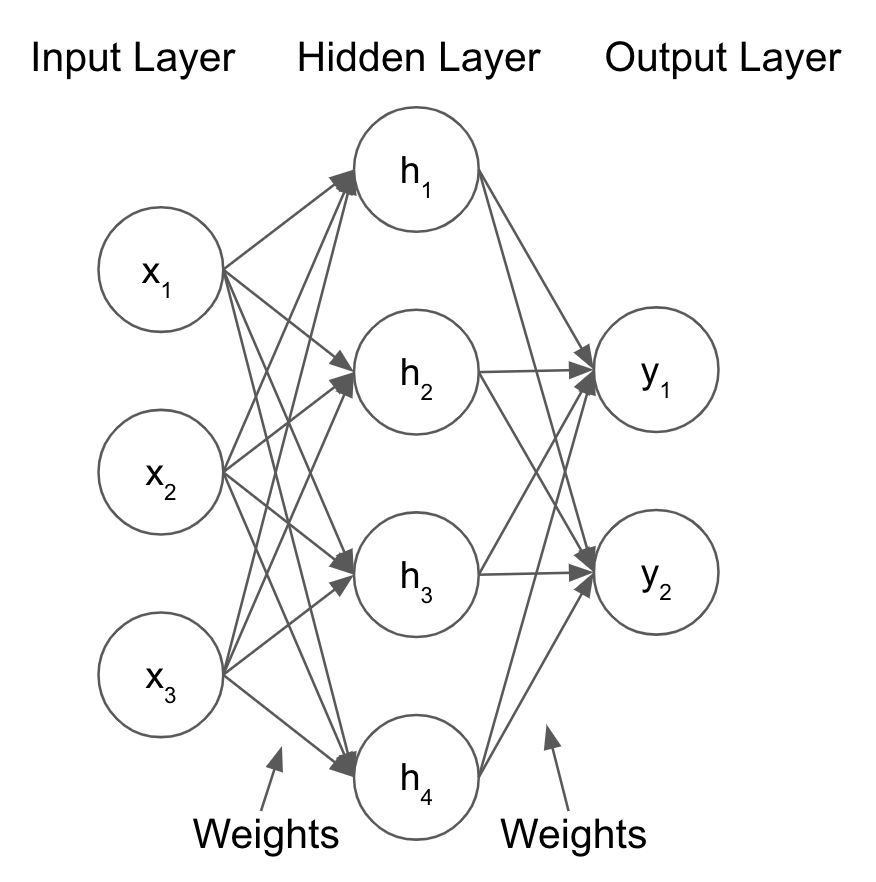
\includegraphics[width=0.5\linewidth]{NeuralNet.png}
		\centering\caption{A simple neural network}
		\label{fig1}
	\end{figure}
	\begin{itemize}
		\item{
			\begin{concept}{Forward Propagation}
				\ \newline
				A series of steps taken by the network to get from inputs to outputs.
				
				Starting with the input $x$, the network computes the net input to the output unit, by calculating the weighted sum
				$$a_j = \sum_{i} w_{ij} x_i$$
				where $w_{ij}$ is the weight from input unit $i$ to hidden unit $j$ and $x_i$ is the input unit $i$.
				
				The hidden layer then applies an activation function $h$ to the weighted sum $a_j$, which gives the activated values $h(a_j)$ at the hidden layer.
				$$h_j = h(a_j)$$
				
				The activated values at the hidden layer are now the input values to the output layer.
				
				The outputs are computed in a similar manner by first computing the weighted sum.
				$$a_k = \sum_{j} w_{jk} z_j$$
				where $z_j = h(a_j)$, the activated value of hidden unit $j$ and $w_jk$ is the weight from hidden unit $j$ to output unit $k$.
				
				The activated outputs are then computed by applying an output activation function, called $y$, to the weighted sum.
				$$y_k = y(a_k)$$

			\end{concept}
		}
		\item{
			\begin{concept}{Backpropagation}
				\ \newline
				A series of steps taken by the network to calculate the gradients at each layer starting from the outputs.
				
				The outputs at the output layer are used to calculate the gradients at the hidden layer, and the gradients at the hidden layer are used to calculate the gradients at the input layer.
				
				What are we taking the gradients of? \textbf{The gradients of the loss function $E$ with respect to the weights.}
				
				Why? \textbf{Because we want to update the weights such that they move in the direction that would minimize the loss function (i.e. Gradient Descent).}
				
				At each layer, we want to calculate the gradient $\frac{\partial E}{\partial w_{ij}}$, which is the same as the product of the delta of the next layer's unit $j$ and the input unit $i$ \textbf{from that layer to the next layer}.
				$$\frac{\partial E}{\partial w_{ij}} = - \delta_j z_i$$

				If $j$ is an output unit, $\delta_j = (t_j - y_j)$.\\
				If $j$ is a hidden unit, $\delta_j = h'(a_j) \sum_{k} \delta_k w_{jk}$, where $h'$ is the derivative of the hidden activation function with respect to the weighted sum $a_j$. 
				
				We can see that we have a recursive definition of $delta$ since each $delta$ is dependent on the next layer's $delta$ values.
			\end{concept}
		}
		\item{
			\begin{concept}{Update Rule}
				\ \newline
				At each layer, the weight is updated using the following equation
				$$w_{ij} = w_{ij} - \alpha \frac{\partial E}{\partial w_{ij}}$$
				or
				$$w_{ij} = w_{ij} + \alpha \delta_j z_i$$
				where $\alpha$ is the learning rate.
				
				Assume we have a neural network with 3 layers as in Figure \ref{fig1} with input unit labeled as $i$, hidden unit labeled as $j$, and output unit labeled as $k$, the update rule at the hidden layer is: 
				$$w_{jk} = w_{jk} + \alpha \delta_k z_j$$
				$$w_{jk} = w_{jk} + \alpha (t_k - y_k) z_j$$
				And the update rule at the input layer is:
				$$w_{ij} = w_{ij} + \alpha \delta_j z_i$$
				or in the unraveled form:
				$$w_{ij} = w_{ij} + \alpha \cdot h'(a_j) \sum_{k} \delta_k w_{jk}$$
				$$w_{ij} = w_{ij} + \alpha \cdot h'(a_j) \sum_{k} (t_k - y_k) w_{jk}$$
			\end{concept}
		}
		\item{
			\begin{concept}{Steps to training a Neural Network}
				\
				\begin{enumerate}
					\item{
						Forward Propagation to calculate the outputs.
					}
					\item{
						Backpropagation using the outputs to calculate the gradients.
					}
					\item{
						Update weights using the gradients calculated.
					}
					\item{
						Repeat 1 through 3 until convergence (loss stops decreasing).
					}
				\end{enumerate}
			\end{concept}
		}
	\end{itemize}
\end{concept}

\begin{concept}{Convolutional Neural Network}
	\
	\begin{itemize}
		\item{
			\begin{concept}{Why Convolution Neural Network?}
				\
				\begin{itemize}
					\item{
						Often used to extract features from images.
					}
					\item{
						Relies on the observation that image's nearby pixels are dependent on each other.
					}
					\item{
						Achieves translational invariance. Objects in the image are independent of where they are placed in the image.
					}
					\item{
						Objects are made of parts. The deeper the CNN goes, the more complex features it could extract.
					}
					\item{
						Resembles the neuroscience concept of \textbf{receptive fields} in the sense that the neurons are stimulated by a restricted region in the image.
					}
				\end{itemize}
			\end{concept}
		}
		\item{
			\begin{concept}{Architecture of a CNN}
				\
				\begin{itemize}
					\item{
						\textbf{Convolutional Layers}
						
						The core of CNN. The layer's weights are filters (or kernels). During the forward propagation, the filters are convolved across the width and height of the input volume.
						
						The convolution is done by computing the dot product between the 2-dimensional patch of the input and the kernel.
					}
					\item{
						\textbf{Pooling Layers}
						
						A form of down sampling the input. The pooling layer often used is max pooling, which uses the maximally activated neuron of each patch as the output.
						
						Pooling helps achieve translational invariance.
					}
					\item{
						\textbf{Activation Layers}
						
						Applies non-linearity to the network. The activation function often used is ReLU. Some other functions are Tanh and Sigmoid.
					}
					\item{
						\textbf{Fully connected layers}
						
						Goes at the end after convolutional layers and pooling layers. This is the "high-level reasoning" layer, which learns non-linear combinations of the high-level features that were output from the previous layers. What it essentially provides to the network is that it learns what features are important from the feature space input.
						
						The fully connected layer is often a linear layer, which has the output
						$$y = xW^T + b$$
						where $W$ is the weight matrix of dimension $(output\_size, input\_size)$, and $b$ is the bias weight of dimension $(output\_size)$.
					}
				\end{itemize}
			\end{concept}
		}
	\end{itemize}
\end{concept}


\end{document}